\begin{figure}
		\begin{footnotesize}
			

		\begin{center} 
		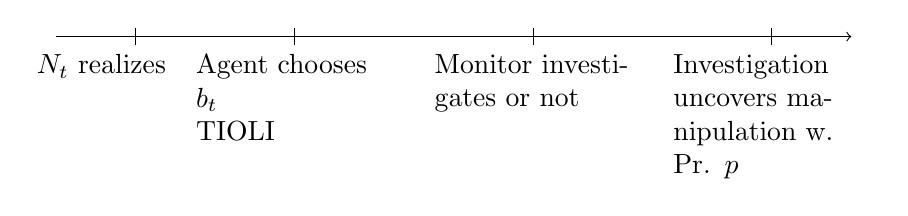
\begin{tikzpicture}[scale=\textwidth/12cm] 
		% draw horizontal line  
		\draw[->] (0,0) -- (10,0);  
		% draw vertical lines  
		\foreach \x in {1,3,6,9}  
		\draw (\x cm,3pt) -- (\x cm,-3pt); 
		% draw nodes  
		\draw (1,0) node[below=3pt,text width=2.5cm] {$N_t$ realizes}; 
		\draw (3,0) node[below=3pt,text width=2.5cm]{Agent chooses $b_t$ \\ TIOLI}; 
		\draw (6,0) node[below=3pt,text width=2.5cm] {Monitor investigates  or not}; 
		\draw (9,0) node[below=3pt,text width=2.5cm] {Investigation uncovers manipulation w. Pr. $p$}; 
		\end{tikzpicture}  
		\end{center} 
		\end{footnotesize} 
\caption{\label{fig:Timeline-bribes}Timeline on $[t,t+h]$}
\end{figure}